\DiaryEntry{Division Theorem, Least Common Multiple, and $ax + by = c$}{2020-08-11}{Category}

\subsection{Division Algorithm}

\begin{theorem}
  Given two integers $a,b$ with $b > 0$, there exist unique integeers $q, r$ satisfying

  \bee
  a = qb + r, \quad 0 \leq r < b
  \eee

  The integer $q$ is called the quotient, the integer $r$ is called the remainder.
\end{theorem}

Intuitively, the theorem is true: The product $qb$ can take on the values $b, 2b, 3b, \dots$ and the value $a$ sits somewhere ``in between''. Since the remainder has to be positive, $q = \lfloor \frac{a}{b} \rfloor$ and the remainder $r$ ``fills up'' the space between $q$ and $a$. If we restrict $r$ to $0 \leq r < b$, then $r,q$ are unique: If $a = qb$, then nothing needs to be filled up, therefore $r = 0$. On the other hand, the largest value for $r$ is when $a = (q+1)b-1$ with $r = b-1$.

This is shown in the following Figure.

\begin{figure}[H]
\centering
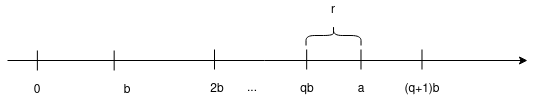
\includegraphics[scale=0.7]{images/division_stuff_1.png}
\end{figure}

\qed

Had we allowed a larger range of $r$; e.g. $0 \leq r < 2b$, there would be two choices for $r$ and $q$: The one from above with $q = \lfloor \frac{a}{b}\rfloor$ and $r = a - qb$ and the second one with $q = \lfloor \frac{a}{b}\rfloor - 1$; i.e. ``one to the left'' and $r = a - qb = a - \lfloor \frac{a}{b}\rfloor b + b$.

The theorem extends naturally to negative values of $b$; in this case

\bee
a = qb + r, \quad 0 \leq r < |b|
\eee

We can use this theorem to show various facts about divisibility of numbers.

\paragraph{Divisibility by $4$.} We first note that a number $n$ is either even or odd; this can be represented as $n = 2q$ and $n = 2q+1$, respectively. The square of the number is then either $4q^2$ or $4q^2 + 4q + 1 = 4(q^2+q) + 1$. From this we can deduce that a squared number is divisible by $4$ with zero remainder or remainder $1$. \qed

As an example, $25 / 4 = 6 \cdot 4 + 1, 36 / 4 = 9 \cdot 4$.

\paragraph{Square of odd Integers.} The square of an odd integer is of the form $8k+1$. We start by representing integers by one of the four forms $4k, 4k+1, 4k+2, 4k+3$. Since $4k$ is even (no matter if $q$ is even or odd), only $4k+1$ and $4k+3$ are odd. Squaring them yields

\bee
(4k+1)^2 = 16k^2 + 8k + 1 = 8(2k^2+k) + 1 = 8 q + 1
\eee

and

\bee
(4k+3)^2 = 16k^2 + 24k + 9 = 8(2k^2 + 3k+1) + 1 = 8q + 1 \qed
\eee

\paragraph{$N = \frac{a(a^2+2)}{3}$ is an Integer.} Same story; we express our integer as one of $3k, 3k+1, 3k+2$. Inserting these three options into the expression yields

\bee
N = \frac{3k(9k^2+2)}{3} = k(9k^2+2),
\eee

and

\bee
N = \frac{(3k+1)((3k+1)^2+2)}{3} = \frac{27k^3 + 27k^2 + 15k+3}{3} = 9k^3 + 9k^2 + 5k + 1,
\eee

and

\bee
N = \frac{(3k+2)((3k+2)^2+2)}{3} = \frac{27k^3 + 54k^2 + 42k+12}{3} = 9k^3 + 18k^2 + 14k + 4.
\eee

It can be seen that all three options yield integer values. \qed

\subsection{Least Common Multiple}

There are three entries related to the GCD: \href{2017-04-26:entry}{this one}, \href{2017-05-01:entry}{this one}, and \href{2017-09-28:entry}{this one}.

Closely related to the GCD is the least common multiple (LCM) of two numbers. An integer $c$ is a \emph{common multiple} of two nonzero integers $a, b$, if $a | c$ and $b | c$. The set of common multiples contains a smallest integer and that's the LCM. The formal definition is as follows.

The LCM $m = \lcm(a,b)$ of two nonzero integers $a, b$ is defined as
\begin{itemize}
\item $a|m$ and $b|m$.
\item If $a|c$ and $b|c$ , with $c > 0$, then $m \leq c$.
\end{itemize}

The following theorem yields a practical way to calculate the LCM.

\begin{theorem}
  For positive integers $a, b$, we have
  \bee
  \gcd(a,b)\lcm(a,b) = ab
  \eee
\end{theorem}

\begin{proof}
  We use $d = \gcd(a,b)$ and write $a = dr, b = ds$ for some integers $r,s$. We further define $m = ab / d$, then $m = dr b / d = rb$ and also $m = a ds / d = as$. Therefore $m$ is is positive common multiple of $a$ and $b$. We want to show that $m$ is the smallest common multiple.

  Now let $c$ be any common multiple of $a$ and $b$; we use $c = au = bv$. From the GCD entries, we know that thee exist integhers $x, y$ such that $\gcd(a,b) = d = ax + by$. Therefore we have

  \bee
  \frac{c}{m} = \frac{cd}{ab} = \frac{c(ax + by)}{ab} = \frac{c}{b}x + \frac{c}{a}y = vx + uy
  \eee

  From this equation we conclude that $c$ is a multiple of $m$; i.e. $m | c$ and therefore $m \leq c$. From the above LCM definition, therefore $m = \lcm(a,b)$, that is

  \bee
  \lcm(a,b) = \frac{ab}{\gcd(a,b)}
  \eee
\end{proof}

The GCD can take on values in the range of $1$ (if $a$ and $b$ are coprime) up to $\min(a,b)$ (when $a$ is a multiple of $b$ or vice versa). Therefore, the LCM can take on values in the range of $\max(a,b)$ (when $a$ is a multiple of $b$ or vice versa) to $ab$ (when $a$ and $b$ are coprime).

\subsection{The Diophantine Equation $ax + by = c$}

The simplest Diophantine equation is the linear equation

\bee
ax + by = c
\eee

where $a, b, c$ are given integers (with $a, b \neq 0$) and we seek integer solutions for $x$ and $y$.

A simple example is $3x + 6y = 18$ which has several integer solutions,

\begin{align*}
  &3 \cdot 4 + 6 \cdot 1 = 18 \\
  & 3 \cdot (-6) + 6 \cdot 6 = 18 \\
  & 3 \cdot 10 + 6 \cdot (-2) = 18
\end{align*}

On the other hand, the equation $2x + 10y = 17$ has no integer solution, as the LHS will always be even.

These observations raise the question, under which conditions the Diophantine equation has a solution. This is answered in the following theorem.

\begin{theorem}
  The linear Diophantine equation $ax + by= c$ has a solution iff $d = \gcd(a,b) | c$. If $x_0, y_0$ is a particular solution of the equation, then all other solutions are given by

  \bee
  x = x_0 + \frac{b}{d}t, \quad y = y_0 - \frac{a}{d}t
  \eee

where $t$ is an arbitrary integer.  
\end{theorem}

\begin{proof}
  Suppose a solution $x_0, y_0$ is known; i.e. $ax_0 + by_0 = c$. Suppose there is a second solution $x', y'$, we have

  \bee
  ax_0 + by_0 = c = ax' + by'
  \eee

  and from which we obtain

  \bee
  a(x' - x_0) = b(y_0 - y')
  \eee

  We know (see for a proof below) that there exist relatively prime integers $r$ and $s$ such that $a = dr, b = ds$. Substituting this into the last equation, we obtain

  \bee
  dr(x' - x_0) = ds(y_0 - y') \rightarrow r(x' - x_0) = s(y_0 - y')
  \eee

  where we have cancelled out the factor $d$ in the last step. From this we deduct $r | s(y_0 - y')$ and since $\gcd(r,s) = 1$, we have $r | (y_0 - y')$ or $rt = y_0 - y'$ for some integer $t$. Substituting, we obtain $x' - x_0 = st$ .

  This yields the following relations

  \begin{align*}
    x' &= x_0 + st = x_0 + \frac{b}{d}t \\
    y' &= y_0 - rt = y_0 - \frac{a}{d}t
  \end{align*}

  If we insert these solutions into the Diophantine equation, we can see that

  \begin{align*}
    ax' + by' &= a \left( x_0 + \frac{b}{d}t \right) + b \left(  y_0 - \frac{a}{d}t \right) \\
              &= ax_0 + by_0 + a \frac{b}{d}t - b \frac{a}{d}t = ax_0 + by_0
  \end{align*}
\end{proof}

\paragraph{Add-on.} If $\gcd(a,b) = d$, then $a/d$ and $b/d$ are coprime; i.e.$\gcd(a/d, b/d) = 1$. Proof: We know that there exist integers $x, y$ so that $ax + by = d$ and therefore $\frac{a}{d}x + \frac{b}{d}y = 1$. Since the $a, b$ are divisible by the gcd, the fractions $\frac{a}{d}$ and $\frac{b}{d}$ are integers and we therefore conclude that $\frac{a}{d}$ and $\frac{b}{d}$ are coprime.

Intuitively, this makes sense as $d$ is the greatest ``something'' we can divide $a$ \emph{and} $b$ by; the remainder is then coprime. \qed

Since we now know how to obtain all solutions once we know one, we need to find a way to find the one solution $x_0, y_0$. The \emph{extended Euclidean Algorithm} additionally provides the numbers $r, s$ for which

\bee
a r + b s = \gcd(a,b)
\eee

holds. The algorithm will be topic of another entry, but we will use it nevertheless. From the above theorem, we know that the linear Diophantine equation $ax + by = c$ has a solution only when $c$ is a multiple of $\gcd(a,b)$; i.e. $ax + by = t \gcd(a,b)$ for some integer $t$. We solve the problem as follows: We first use the extended Euclidean algorithm to obtain $r, s$ from

\bee
a r + b s = \gcd(a,b)
\eee

The we multiply both sides with $t$ and obtain

\bee
a (rt) + b (st) = t \gcd(a,b)
\eee

from which we deduce the solution

\bee
x_0 = rt, y_0 = st .
\eee

\paragraph{Example.} We consider the example from above, $3x + 6y = 18$. We have $\gcd(3,6) = 3$, and since $3 | 18$ the equation has inifitely many solutions. The extended Euclidean algorithm applied to

\bee
3 r + 6 s = 3
\eee

yields $r = 1, s = 0$; i.e. $3 \cdot 1 + 6 \cdot 0 = 3$. Multiplying both sides with $c / \gcd(a,b) = 18 / 3 = 6$ yields

\bee
3 \cdot 1 \cdot 6 + 6 \cdot 0 \cdot 6 = 18
\eee

from which we obtain our particular solution as $x_0 = 6, y_0 = 0$. The solutions are therefore

\begin{align*}
  x &= x_0 + \frac{6}{3}t = 6 + 2t \\
  y &= y_0 - \frac{3}{3}t = -t
\end{align*}


As another example, we consider $8x + 34y = 16$. The gcd equals $\gcd(8, 34) = 2$ and $2 | 16$, so there exist solutions. Solving $8r + 34s = 2$ via the extended Euclidean algorithm yields $r = -4, s=1$, so we can write

\bee
8 \cdot (-4) + 34 \cdot 1 = 2
\eee

Multiplication of both sides by $8$ yields

\bee
8 \cdot(-32) + 34 \cdot 8 = 16
\eee

from which we obtain $x_0 = -32, y_0 = 8$. Our solutions therefore are
\begin{align*}
  x &= x_0 + \frac{34}{2}t = -32 + 17t \\
  y &= y_0 - \frac{8}{2}t = 8 - 4t
\end{align*}

%%% Local Variables:
%%% mode: latex
%%% TeX-master: "journal"
%%% End:
